\newcommand{\jp}{j^\prime}
\newcommand{\jpp}{j^{\prime\prime}}
\newcommand{\lp}{l^\prime}
\newcommand{\lpp}{l^{\prime\prime}}
\newcommand{\fc}{\bm{\Phi}\genfrac{(}{)}{0pt}{}{j \jp}{l \lp}}
\newcommand{\fczero}{\bm{\Phi}\genfrac{(}{)}{0pt}{}{j \jp}{0 \lp}}
\newcommand{\fcb}{\bm{\Theta}\genfrac{(}{)}{0pt}{}{j \jp}{l \lp}}
\newcommand{\fcbpp}{\bm{\Theta}\genfrac{(}{)}{0pt}{}{j \jpp}{l \lpp}}
\newcommand{\fcbf}{-\bm{\Theta}\genfrac{(}{)}{0pt}{}{j \jp}{l \lp} + \delta_{j,\jp} \delta_{l,\lp} \sum_{\jpp, \lpp}  \bm{\Theta}\genfrac{(}{)}{0pt}{}{j \jpp}{l \lpp} }
\newcommand*\tageq{\refstepcounter{equation}\tag{\theequation}}

\chapter{Simulation methods}

\section{Density Functional Theory}\label{sec:dft}

\subsection{The many-body wavefunction}
In electronic structure calculations we are ultimately interested in the many-body wavefunction

\[ \Psi(\bm{r}_1,\bm{r}_2,\dots, \bm{r}_n; \bm{R}_1, \bm{R}_2, \dots , \bm{R}_N) \]

\noindent where $\bm{r}_i$ are electron coordinates and $\bm{R}_i$ are nuclear coordinates. Imagine that we want to calculate this object for a small molecule such as Benzene (C$_6$H$_6$) containing 12 nuclei and 42 electrons. This wavefunction exists in $42\cdot3-6 = 156$ dimensional cartesian space! If we want to store this object on a computer with a modest precision of 10 grid points per coordinate, it would require $10^{156}$ complex numbers or $64 \cdot 10^{156}$ bits (assuming single-precision floating points numbers of 32 bits). Lloyd2000 estimated the total number of bits available for computation in the observable universe to be $10^{90}$ (Lloyd2000). Even with the entire universe at our disposal this object is completely unmanageable. This exercise also emphasizes the potential of Quantum Computers. For this reason, we fix the ionic positions and assume that the many-body wavefunction can be written as a product of single-electron wavefunctions (orbitals):

\[ \Psi(\bm{r}_1,\bm{r}_2,\dots, \bm{r}_n; \bm{R}_1, \bm{R}_2, \dots , \bm{R}_N) \longrightarrow \phi(\bm{r}_1)\phi(\bm{r}_2)\dots\phi(\bm{r}_n) \]

\subsection{The Kohn-Sham equations}

\subsection{The Hellman-Feynman theorem and molecular forces}

\subsection{DFT+U}

\section{Phonon calculation formalism}
In most textbooks (e.g. Kittel \cite{Kittel2005}), phonon calculations are exemplified by simple models in one dimension consisting of only one or two inequivalent atoms. While these models are useful for providing basic results of lattice dynamical models, the extension to realistic models requires some level of abstraction in order to be useful. In particular, it is essential to cast the problem in terms of linear algebra. In this section, I will start from the (somewhat abstract) formalism used in practice and work backwards towards a physical understanding. While software such as PHONON \cite{Parlinski1997} and Phonopy \cite{Togo2015} can be used without prior knowledge of the formalism, it is always useful to have some insights about our frequently used 'black boxes`. In order to calculate the phonon spectrum for a given system in the harmonic approximation, we require the following objects:

\begin{enumerate}
	\item Primitive unit cell and fractional atomic coordinates
	\item Symmetry operations
	\item The mass of each atomic species
	\item The force constants
\end{enumerate}

Items 1-3 are familiar to most condensed matter physicists and can usually be found in various databases. The force constants, on the other hand, contains information about interatomic forces and is not directly obtainable from experiment. For this reason, phonon calculations requires some modelling either through semi-empirical or ab-initio methods. In the following I will attempt to explain what the force constants represents and how we use them to get phonon band structures.

\subsection{Theory}

We start completely generally in one dimension with an arbitrary number of unit cells containing an arbitrary number of atomic species at equilibrium. Displacements from equilibrium positions are denoted $u(jl)$, where $l$ is the unit cell index and $j \in \{1,\dots,n\}$ is the atomic index. If we consider the displacements $u$ to be small, the total energy of our system can be expressed as a Taylor series

\[ E^\text{tot} = E_0 + \sum_{l}\sum_{j} \left. \frac{\partial E}{\partial u(jl)} \right\rvert_{r_{lj}}  + \frac{1}{2} \sum_{l,\lp} \sum_{j,\jp} u(jl) \left. \frac{\partial ^2 E}{\partial u(jl) \partial u(\jp \lp)} \right\rvert_{r_{lj}, r_{\lp \jp}} u(\jp \lp) + \dots \, , \]

\noindent where $r_{lj}$ is the equilibrium position of atom $j$ in unit cell $l$. The main approximation in phonon calculations is the so-called \emph{harmonic approximation} which ignores terms with power greater than 2 in the series. Higher-order contributions are denoted \emph{anharmonic} terms and can become important at higher temperatures (phase transitions, thermal conductivity, thermal expansion). The fact that our system is in equilibrium can be stated succinctly as

\[ \frac{\partial E}{\partial u(jl)} = 0 \, , \]

\noindent for all values of $j$ and $l$. Physically these assumptions together correspond to atoms being at rest in a parabolic (harmonic) potential. Since we are interested in  dynamics, it is convenient to consider the \emph{harmonic energy} $E$ of the system

\begin{equation}
E = E^\text{tot} - E_0 = \frac{1}{2} \sum_{l,\lp} \sum_{j,\jp} u(jl) \left. \frac{\partial ^2 E}{\partial u(jl) \partial u(\jp \lp)} \right\rvert_{r_{lj}, r_{\lp \jp}} u(\jp \lp) \label{eq:eharm}
\end{equation}

\noindent If we set $j=\jp$ and $l=\lp$, we see that the harmonic energy of a single atom has the familiar form of a harmonic oscillator $E=\frac{1}{2}Ku^2$, where $K$ is the spring constant. We define

\[ \left. \frac{\partial ^2 E}{\partial u(jl) \partial u(\jp \lp)} \right\rvert_{r_{lj}, r_{\lp \jp}} = \fc = \fcbf \]

\noindent where $\bm{\Phi}$ is the called the \emph{force constant} with respect to total energy and $\bm{\Theta}$ is the force constant with respect to bond energy. We can now write the harmonic energy as

\begin{align*}
E &= \frac{1}{2} \sum_{l,\lp} \sum_{j,\jp} u(jl) \fc u(\jp \lp) \tageq\label{eq:total_energy} \\
&= \frac{1}{2} \sum_{l,\lp} \sum_{j,\jp} u(jl) \left( \fcbf \right) u(\jp \lp) \\
&= \frac{1}{2} \sum_{l,\lp} \sum_{j,\jp} \left( - \fcb u(jl)u(\jp,\lp) + \fcb u(jl)^2 \right) \\
&= \frac{1}{2} \sum_{l,\lp} \sum_{j,\jp} \left( - \fcb u(jl)u(\jp,\lp) +\frac{1}{2} \fcb \left( u(jl)^2 + u(\jp, \lp)^2 \right) \right) \\
&= \frac{1}{4} \sum_{l,\lp} \sum_{j,\jp} \fcb \left[ -2u(jl)u(\jp,\lp) + u(jl)^2 + u(\jp,\lp)^2 \right] \\
&= \frac{1}{4} \sum_{l,\lp} \sum_{j,\jp} \fcb \left[ u(jl) - u(\jp,\lp) \right]^2
\end{align*}

\begin{figure}
	\centering
	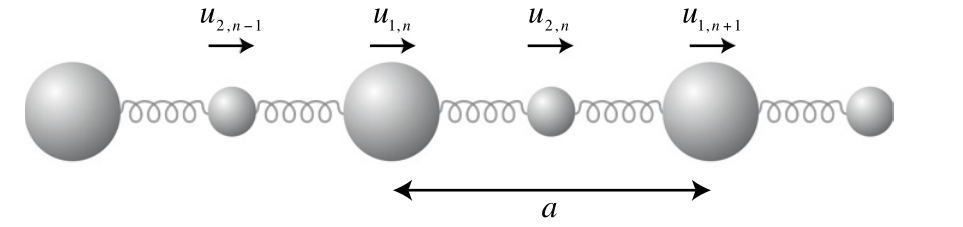
\includegraphics[width=0.9\textwidth]{fig/temp/diatomic.png}
	\caption[diatomic chain]{Diatomic chain. \todo[inline]{Make new figure. Use $l$ as unit cell index for consistency with the notation.}}
	\label{fig:diatomic}
\end{figure}

\noindent and it becomes evident that the harmonic energy can be described with respect to atoms or bonds in mathematically equivalent ways. Since the bond-centered description does not include individual atomic displacements, it is necessary to add a self-term to $\bm{\Theta}$. As a visual aid to these index-heavy equations, Figure \ref{fig:diatomic} illustrates the one-dimensional diatomic chain, which is often used in introductory texts. If we consider only nearest-neighbour interactions and identical springs, the bond-centered harmonic energy can be written

\begin{align*}
E &= \frac{1}{4} \bm{\Theta} \sum_l 2 \left[ u(1,l) - u(2,l) \right]^2 + \frac{1}{4} \bm{\Theta} \sum_n 2 \left[ u(2,l) - u(1,l+1) \right]^2 \\
&= \frac{1}{2} \bm{\Theta} \sum_l \left[ u(1,l) - u(2,l) \right]^2 + \frac{1}{2} \bm{\Theta} \sum_n \left[ u(2,l) - u(1,l+1) \right]^2
\end{align*}

\noindent where the factor of 2 comes from double-counting. The purpose of this example is to show that the (somewhat abstract) harmonic energy in equation \eqref{eq:eharm} is equivalent to our intuitive understanding of coupled harmonic oscillators. With this in mind, we can return to the matter at hand and write the equation of motion for an atom $j$ in cell $l$ through Newtons second law $F=ma$:

\[ m_j \ddot{u}(jl, t) = - \frac{\partial E}{\partial u(jl)} = - \sum_{\lp} \sum_{\jp} \fc u(\jp \lp, t) \, , \]

\noindent where $m_j$ is the atomic mass of atom $j$\todo{Where does the factor 2 come from when taking the derivative?!?}. Solutions to this equation is given as a sum of travelling harmonic waves with wave vectors $q$ and band indices $\nu \in \{1,\dots , n \}$

\[ u(jl,t) = \sum_{q,\nu} \tilde{u}(j,q,\nu) \exp (iqr(jl)) \exp(-i \omega(q,\nu) t) \, \]

\noindent where $\omega(q,\nu)$ is the frequency, $r(jl)$ is the position of atom $j$ in cell $l$ and  is the frequency and the complex number $\tilde{u}$ is called the \emph{displacement vector}. If we insert these solutions into the equations of motion and just consider one band at one wave vector we obtain

\begin{align*}
m_j \omega(q,\nu)^2 \tilde{u}(j,q,\nu) \exp(ikr(jl)) &= - \sum_{\lp} \sum_{\jp} \fc \tilde{u}(\jp,q,\nu) \exp (ikr(\jp\lp)) \\
m_j \omega(q,\nu)^2 \tilde{u}(j,q,\nu) & = - \sum_{\lp} \sum_{\jp} \fc \tilde{u}(\jp,q,\nu) \exp (ik[r(\jp\lp) - r(jl)]) \\
m_j \omega(q,\nu)^2 \tilde{u}(j,q,\nu) & = - \sum_{\lp} \sum_{\jp} \fczero \tilde{u}(\jp,q,\nu) \exp (ik[r(\jp\lp) - r(j0)]) \tageq\label{eq:motion} \, ,
\end{align*}

\noindent where the last equality is simply a change of origin in order to follow the convention of most software. The full account of phonon frequencies $\omega$ and displacements $\tilde{u}$ can be found as a solutions to equation \eqref{eq:motion}. At a given $q$ and $\nu$, the equations are indexed by $j$ and we will have $n$ equations with $n$ unknowns with respect to $\tilde{u}(j,q,\nu)$, where $n$ is the number of atoms in the unit cell. In fact, equation \eqref{eq:motion} can be written as an eigenvalue equation:

\begin{equation}
\bm{D}(q) \cdot \bm{e}(q,\nu) = \omega(q,\nu)^2 \cdot \bm{e}(q,\nu) \, , \label{eq:dynmat}
\end{equation}

\noindent where 

\[ \bm{e}(q,\nu) = \begin{pmatrix}
\sqrt{m_1}\tilde{u}(1,q,\nu) \\
\sqrt{m_2}\tilde{u}(2,q,\nu) \\
\vdots \\
\sqrt{m_n}\tilde{u}(n,q,\nu)
\end{pmatrix} \]

\noindent and the elements of $\bm{D}(q)$ are given 

\begin{equation}
D(j\jp) = \frac{1}{\sqrt{m_j m_{\jp}}} \sum_{\lp} \fczero \exp (iq[r(\jp\lp) - r(j0)]) \, . \label{eq:dynmat_ij}
\end{equation}

\noindent $\bm{D}(q)$ is known as the dynamical matrix and can be constructed solely from force constants. Furthermore, equation \eqref{eq:dynmat_ij} reveals that the dynamical matrix is Hermitian so the eigenvalues $\omega(q,\nu)^2$ are real and the eigenvectors $\bm{e}(q, \nu)$ are orthonormal. In addition, the eigenvalues and eigenvectors are trivially obtained numerically (e.g. \texttt{numpy.linalg.eigh} in the Python numpy library). In order to get the full dispersion, this diagonalization is performed for each of the $n$ bands $\nu$ at the desired wave vectors in the first Brillouin Zone (FBZ). 

The extension to 3 dimensions is done by treating the Cartesian components separately and considering $\bm{q}$ and $\bm{r}$ as vectors. The eigenvector then becomes a column vector of $3n$ components 

\[ \bm{e}(\bm{q},\nu) = \begin{pmatrix}
\sqrt{m_1}\tilde{u}_x(1,\bm{q},\nu) \\
\sqrt{m_1}\tilde{u}_y(1,\bm{q},\nu) \\
\sqrt{m_1}\tilde{u}_z(1,\bm{q},\nu) \\
\sqrt{m_2}\tilde{u}_x(2,\bm{q},\nu) \\
\vdots \\
\sqrt{m_{n}}\tilde{u}_z(n,\bm{q},\nu)
\end{pmatrix} \, , \]

\noindent the number of bands increase to $3n$ and we get a $3n \times 3n$ dynamical matrix, where each component \eqref{eq:dynmat_ij} is a $3 \times 3$ block of the form

\[
\bm{D}(j\jp) = \begin{pmatrix}
D(j\jp)_{xx} & D(j\jp)_{xy} & D(j\jp)_{xz} \\
D(j\jp)_{yx} & D(j\jp)_{yy} & D(j\jp)_{yz} \\
D(j\jp)_{zx} & D(j\jp)_{zy} & D(j\jp)_{zz}
\end{pmatrix}
\]

\noindent where

\begin{equation}
D(j\jp)_{\alpha\beta} = \frac{1}{\sqrt{m_j m_{\jp}}} \sum_{\lp} \fczero _{\alpha\beta} \exp (i\bm{q}[\bm{r}(\jp\lp) - \bm{r}(j0)]) \label{eq:dynmat_ij2}
\end{equation}

\noindent While the path was somewhat involved, it is useful to take a step back and consider the consequences of our outlined formalism. Everything we need to know about our phonon system can be obtained from the dynamical matrix that, in turn,  is constructed from force constants through equation \eqref{eq:dynmat_ij2}. Finally, all of these objects can be constructed in computationally trivial way from force constants.

\subsection{Practical considerations}\label{sec:phononpractical}
At this point, it is useful to consider how we construct elements of the dynamical matrix in practice. Inspection of equation \eqref{eq:dynmat_ij2} contains a sum over all unit cells $\lp$ and is thus an infinite sum. On the other hand, it is reasonable to assume that the dominant force constants $\bm{\Phi}$ are short range. The compromise is to use a finite supercell such that the second derivatives involved in calculating force constants outside this cell are minimized. While the reasonable size of such a supercell obviously depends on the system and model, quantum contributions to the force constants generally vanish within a distance of roughly \SIrange{10}{15}{\angstrom} \todo{CRYSTAL website reference? Maybe something better}. If the force constants can be obtained analytically from a semi-empirical potential, calculation is computationally simple and we can use large supercells. However, since force constants are usually obtained from DFT, we are limited by computational resources and are usually restricted to supercells with a maximal interatomic distance of roughly \SI{5}{\angstrom} (e.g. a cubic system with $a=\SI{10}{\angstrom}$).

Since the number of force constants needed is at least equal to the size of the dynamical matrix, the number of calculations to perform is at least $3n \times 3n$. Even for a fairly small system such as LCO in the I4/mmm space group (HTT, $n=7$) the number of elements in the dynamical matrix is $(3\cdot 7)^2 = 441$. In the finite displacement method, each force constant is the result of a self-consistent DFT calculation, so the computational effort appears prohibitively expensive at first glance. For this reason we use a numerical fitting of symmetry inequivalent force constants (see section \ref{sec:forceDFT}). In the case of LCO in the I4/mmm space group the number of necessary displacements is reduced to only 7 (6 if we ignore magnetism), making the problem much more manageable.

\subsection{Phonon eigenvectors}
The phonon dispersion is contained within the eigenvalues $\omega (\bm{q},\nu)^2$. We can plot the bands $\nu$ along high-symmetry lines in the FBZ by carefully choosing the values of $\bm{q}$ where the dynamical matrix is diagonalized. Similarly, we can sample the dispersion in a dense $\bm{q}$-mesh in order to evaluate the phonon density of states. In addition, many thermodynamic properties can be calculated by only considering the eigenvalues.

The eigenvectors $\bm{e}(\bm{q}, \nu)$ are more subtle in nature. Each component of  $\bm{e}(\bm{q}, \nu)$ is a complex number that describes the wave amplitude and phase of one atomic species $j$ in one cartesian direction $\alpha$. In addition, the eigenvector is normalized and thus only describes relative atomic motion. In order to visualize the collective displacement due to a phonon mode $\nu$ at $\bm{q}$ we can displace all atoms $j$ in unit cells $l$ by

\begin{equation}
\Delta_{jl} = \frac{A}{\sqrt{m_j}} \text{Re} \left[ \exp (i\phi) \bm{e}_j(\bm{q}, \nu) \exp (i \, 2 \pi \, \bm{q} \cdot \bm{r}(jl) \right] \label{eq:displacements}
\end{equation}

\noindent where $\bm{e}_j(\bm{q}, \nu)$ is the $j$'th component of $\bm{e}(\bm{q}, \nu)$ and $A$ is an arbitrary amplitude. The phase $\phi$ describes periodic motion of atoms. An animation can be produced by varying $\phi$ between 0 and $2 \pi$.

In \texttt{Phonopy} the eigenvectors are always given with respect to the primitive unit cell and the 3 Cartesian components are along the basis vectors of this primitive unit cell. If we want to, for example, to visualize the bond-stretching mode in the HTT phase of LCO at $q=(\frac{1}{4},\frac{1}{4},0)$ in orthorhombic notation, we look at atoms in primitive unit cells with origin (0,0,0), (1,0,1), (2,0,2) and (3,0,3) using the eigenvectors at $q=(0.125,-0.125,0.125)$. For this specific mode, the movement of oxygen with fractional coordinates (0.5,0,0.5) dominates. The movement is exactly along the Cu-O bond and we can plot it in one dimension. Figure \ref{fig:bs-displacements} shows this phonon mode at the zone center, the zone boundary and halfway through the zone (where the giant phonon anomaly is observed).

\begin{figure}
	\centering
	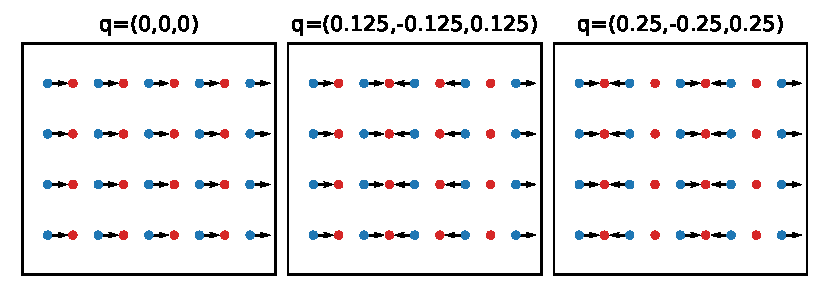
\includegraphics{fig/temp/bs-phonons.pdf}
	\caption[bond-stretching phonons visualized]{Cu-O bond stretching mode in LCO at three different values of $q$ referring to the primitive HTT (I4/mmm) unit cell. Blue markers are oxygen and red markers are copper. The phase is set to $\phi=\frac{3}{4}\pi$ in equation \ref{eq:displacements} in order to get displacement vectors of equal length.}
	\label{fig:bs-displacements}
\end{figure}

\subsection{Obtaining Force Constants from DFT}\label{sec:forceDFT}
Force constants from DFT are found in a surprisingly simple way. In the previous sections we defined the force constant with respect to total energy as

\[ \fc  _{\alpha \beta} = \frac{\partial ^2 E}{\partial u_\alpha (jl) \partial u_\beta (\jp \lp)} = - \frac{\partial F_\beta (\jp \lp)}{\partial u_\alpha (jl)} \]

\noindent where $F_\beta (\jp\lp)$ is the force on atom $(\jp \lp)$ in the direction $\beta$. Notice that everything is now labelled by a Cartesian direction and these directions are treated individually. In practice the Cartesian directions correspond to the unit cell vectors, but to reduce confusion we use the labels ($x,y,z$). We can approximate the derivative by performing a finite displacement $\Delta u_\alpha(jl)$ and simply taking the numerical derivative


\begin{equation}
\fc _{\alpha \beta} \approx - \frac{F_\beta (\jp \lp; \Delta u_\alpha (jl)) - F_\beta (\jp\lp)}{\Delta u_\alpha (jl)} \label{eq:finite}
\end{equation}


\noindent where $F_\beta (\jp\lp;\Delta u_\alpha (jl))$ is the force on atom $(\jp \lp)$ in the direction $\beta$ after performing the displacement $\Delta u_\alpha (jl)$. At equilibrium we assume $F_\beta (\jp \lp) = 0$ and we only need to calculate the forces due to a finite displacement. In ab-initio methods, there is no reason to assume a particular shape of the potential energy landscape and we can only expect the harmonic approximation to be valid for small finite displacements. For this reason, displacements have to be chosen large enough so that we are not subject to numerical noise and small enough to avoid anharmonic contributions. In \texttt{Phonopy} the default value is \SI{0.01}{\angstrom}, while \texttt{PHONON} uses \SI{0.03}{\angstrom}.

As mentioned in section \ref{sec:phononpractical}, we need a large number of force constants to construct the dynamical matrix, even when dealing with small systems. For this reason, a numerical fitting of forces and displacements, known as the Parlinski-Li-Kawazoe method \cite{Parlinski1997}, is used to find force constants. We notice that equation \eqref{eq:finite} can be written as a matrix equation for one pair of atoms $(jl)$ and $(\jp \lp)$:

\[ \bm{F}(\jp \lp) = -\bm{U}(jl) \bm{P} (jl;\jp \lp) \, , \]

\noindent where

\[ \bm{F}(\jp \lp) = (F_x \quad F_y \quad F_z) \, , \]

\[ \bm{U}(jl) = \left( \Delta u_x(jl) \quad \Delta u_y(jl) \quad \Delta u_z(jl) \right)  \]

\noindent and

\[ 
\bm{P} (jl;\jp \lp) = 	
\begin{pmatrix}
\Phi_{xx} & \Phi_{xy} & \Phi_{xz} \\
\Phi_{yx} & \Phi_{yy} & \Phi_{yz} \\
\Phi_{zx} & \Phi_{zy} & \Phi_{zz} 
\end{pmatrix}
\]

\noindent If we perform $m$ finite displacements, we get $m$ simultaneous equations for each pair of atoms:

\begin{equation*}
\begin{pmatrix} \bm{F}_1(\jp\lp) \\ \bm{F}_2(\jp\lp) \\ \vdots \\ \bm{F}_m(\jp\lp) \end{pmatrix} =
- \begin{pmatrix} \bm{U}_1(jl) \\ \bm{U}_2(jl) \\ \vdots \\ \bm{U}_m(jl) \end{pmatrix} \bm{P}(jl;\jp \lp) \, .
\end{equation*}

\noindent which can be solved by a Moore-Penrose pseudo-inverse matrix (in Numpy: \texttt{numpy.linalg.pinv}) given a sufficient number of displacements. Since $\bm{U}$ only depends on $(jl)$, we can build up the full force constant matrix by iterating this procedure over $(\jp \lp)$. The minimum number of displacements is equal to the number of non-equivalent atoms in the crystal primitive unit cell multiplied by a number of independent x,y,z coordinates in the site symmetry of a given atom \cite{Parlinski1997}. For this reason, software such as \texttt{Phonopy} and \texttt{PHONON} determines the primitive unit cell, the supercell expansion matrix and all the symmetry operations before generating displacements.

\section{Molecular Dynamics}
Temperature fluctuations in a closed system:

\[ \frac{\Delta T}{T} = \sqrt{\frac{2}{3N}} \quad \Rightarrow \quad \Delta T(T=\SI{300}{\kelvin}) = \SI{23.1}{\kelvin} \]

\noindent Nose-Hover algorithm:

\begin{align*}
v_i^\text{scaled} &= \frac{\bm{p}_i}{m_i} \\
\text{d}\bm{p}_i &= (\bm{F}_i - \zeta \bm{p}_i) \text{d}t \\
\text{d}\zeta &= \frac{1}{Q} \left( \sum_{i=1}^N \frac{|\bm{p_i}|^2}{m_i} - (3N+1)k_\text{B}T\right) \text{d}t
\end{align*}

\chapter{Experimental Methods}
\section{Neutron Scattering}
\section{X-ray spectroscopy}